\section {Блоки памʼяті}

Блоками памʼяті в цьому програмному рішенні є набором байт, які обробляються системою як єдина одиниця. Розмір блоку складає 4 мегабайти за замовчуванням або розмір вказаний користувачем при розгортанні системи. Як і в деяких існуючих реалізаціях, ціль використання блоків полягає в обʼєданні невеликих фрагментів памʼяті у більш великі блоки для більш швидкої та ефективної обробки, зниження затримки в операцій читання та запису.
	Кожному блоку памʼяті призначається унікальний ідентифікатор (ID), який є цілим числом, яке займає 64 біти памʼяті.

\section {Cервіс зберігання блоків}

Сервіс зберігання блоків - сервіс, що розгортається на вузлах розподіленої системи, що містять вільну памʼять для надання доступу до неї по мережі.
	Інтерфейсом цього компоненту є сховище ключ-значення, де ключем є ідентифікатор блоку памʼяті, а значенням - байти блоку.

\section {Сервіс керування кластером}

Сервіс керування кластером приймає від розгорнутих сервісів зберігання блоків інформацію про кількість блоків, яку вони можуть отримати для зберігання. Далі, за запитами від клієнтських інтеграцій, сервіс керування кластером призначає їм ідентифікатори блоків для використання в клієнтському програмному забезпеченні, а також адреси сервісів зберігання блоків, на яких вони розміщені.
	Для забезпечення відмовостійкості, користувач обирає один зі способів забезпечення відновлення даних у разі програмних чи апаратних збоїв:
Реплікація (за вказаним користувачем фактором n) - цей алгоритм створює n ідентичних копій даних на різних вузлах системи. У разі якщо один з вузлів вийде з кластеру, то дані будуть відновлені з інших вузлів, де зберігаються репліковані копії.
Кодування стиранням (erasure coding) - цей алгоритм ділить блоки даних на менші блоки, кожен з яких має надмірність (конфігурація алгоритму задається користувачем в залежності від його вимог до відмовостійкості кластеру). У разі відмови одного з вузлів кластеру, втрачену інформацію можна відновити з інших частин виконавши нескладні математичні перетворення.
Сервіс керування кластером також надає інструменти для моніторингу, перегляду стану компонентів та внесення змін в кластер. Надається веб-інтерфейс користувача для перегляду інформації. Для інтеграції з зовнішньою системою моніторинга надається HTTP інтерфейс для передачі метрик та статистики у форматі Prometheus.
Крім цього, на сервісі керування кластером полягає роль автоматичної зміни конфігурації кластеру на основі статистики зібраної клієнтськими інтеграціями. Ці налаштування мають вид правил, які відправляються на клієнтські інтеграції та задають їм за яких умов необхідно виконати предзавантаження окремих блоків даних для зниження часу затримки.

\section {Клієнтська інтеграція}

Як зазначалось раніше, клієнтська інтеграція має два варіанти для розгортання на вибір користувача (в кластері можно використовувати обидва одночасно).

\subsection{Бібліотека на мові програмування Rust для інтеграції в клієнтське програмне забезпечення}

Цей спосіб використання підходить для програмного забезпечення, код якого є можливість змінити та яке написане на мові програмування Rust. Ця інтеграція є рекомендованою для використання, оскільки більш ефективна в роботі та має більш низькі затримки.
	Для її використання, користувач додає в своє програмне забезпечення бібліотеку, яка надає йому наступні інструменти для використання в своєму коді:
Розумний показчик FarMemory<T>, який за допомогою механізмів Deref<T> та Drop<T>, наданих мовою програмування Rust, завантажує дані та відправляє до віддаленою памʼяті за необхідністю.
Структура даних FarMemoryList<T> яка реалізує інтерфейс списку та зберігає дані у віддаленій памʼяті
Структура даних FarMemoryTable<K, V> яке реалізує інтерфейс хеш-таблиці та зберігає дані у віддаленій памʼяті
Функцію allocate\textunderscore far\textunderscore memory\textunderscore block, яка резервує блок у віддаленій памʼяті та повертає його ідентифікатор. Ця функція призначена для випадків коли розробнику потрібен низькорівневий доступ до памʼяті.
Функції read\textunderscore far\textunderscore memory\textunderscore block та write\textunderscore far\textunderscore memory\textunderscore block що дозволяють прочитати та записати зміст блоку у віддаленій памʼяті за його ідентифікатором. Ці функція призначена для випадків коли розробнику потрібен низькорівневий доступ до памʼяті.
Функція free\textunderscore far\textunderscore memory\textunderscore block, що визволяє з використання блок памʼяті за його ідентифікатором. Ця функція призначена для випадків коли розробнику потрібен низькорівневий доступ до памʼяті.

\subsection {Сервіс клієнтської інтеграції}

Цей варіант використання призначено для випадків, коли немає можливості змінити програмний код клієнтського програмного забезпечення, або коли воно використовує інші мови програмування, що не дозволяє використати бібліотеку клієнтської інтеграції.

Цей спосіб полягає в розгортанні сервісу на тому ж обладнанні, яке виконує програмне клієнтське програмне забезпечення. Сервіс використовує відповідний функціонал операційної системи Linux для створення віртуального блокового пристрою. Далі цей блоковий пристрій використовується клієнтським забезпеченням для прямого зберігання даних (за необхідністю, на блоковому пристрою розміщується файлова система) або на блоковому пристрою розміщується файл підкачки, в який операційна система при низькому рівні вільної памʼяті, автоматично переносить сторінки памʼяті.

\section {Взаємодія компонентів}

Для комунікації між компонентами використовується TCP/IP зʼєднання. Для кодування повідомлень має сенс використати Protocol Buffers. Це дозволить пересилати дані між компонентами з низькими затримками та додатковими витратами.

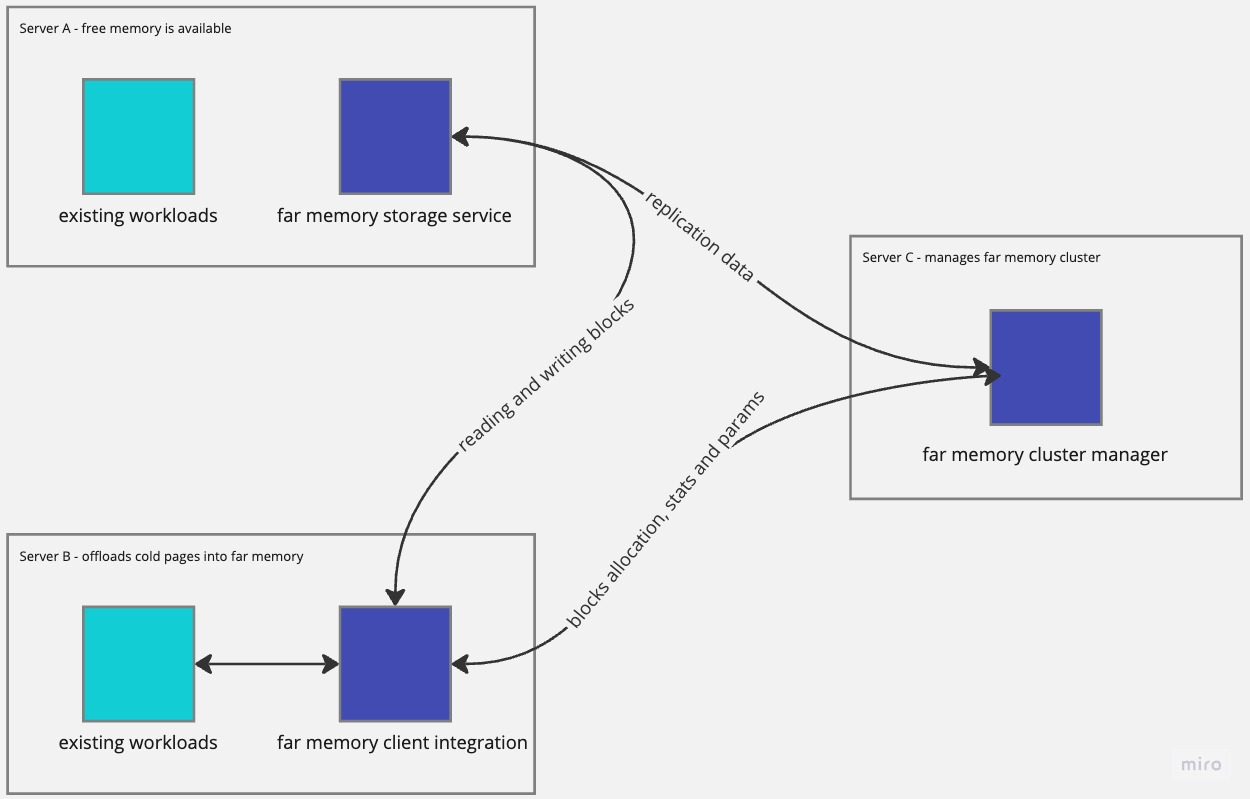
\includegraphics[width=5cm, height=4cm]{image2.jpg}

Рисунок 2.1 - Схема компонентів кластеру та потоки даних між ними.

\section{ВИСНОВКИ}

В цьому розділі було формалізовано вимоги до програмного рішення, що розглядається в межах цього курсового проекту. Грунтуючись на цих вимогах, було розроблено архітектуру програмно визначеної віддаленої памʼяті призначеної для розгортання у сучасних розподілених системах. Ця архітектура та описані деталі її реалізації будуть в подальшому використовуватись при реалізації, тестуванні та впровадженні цього програмного рішення.

\chapter{ВИСНОВОК}

Як підсумок проведеного аналізу проблеми, існуючих досліджень та реалізації та розробки архітектури архітектури програмного рішення програмно-визначеної віддаленої памʼяті, що розглядається у межах цієї роботи, було зроблено декілька висновків.
По-перше, реалізація кластеру віддаленої памʼяті повинна містити наступні компоненти: сервіс керування кластером, сервіс зберігання даних та клієнтська інтеграція. Ці компоненти пересилають блоки памʼяті мережею для переміщення холодних сторінок памʼяті у віддалену памʼять та у зворотному порядку.
По-друге, було встановлено, що найбільш оптимальним методом інтеграції в клієнтське програмне забезпечення є створення бібліотеки яка надає розробникам функції та структури даних для використання в своєму програмного забезпеченні. Також, оскільки велика частка програмного забезпечення не може змінюватись або не підходить до інтеграції з клієнтською бібліотекою за будь-яких причин, було досліджено та реалізовано у архітектурі альтернативний шлях реалізації: за допомогою віртуального блокового пристрою створеного за допомогою відповідного функціоналу операційної системи Linux.
По-третє, були визначені та додані в архітектуру засоби забезпечення відмовостійкості системи та низької затримки операцій читання та запису у віддалену памʼять.
В подальшому, розроблені вимоги та архітектура будуть використані для реалізації програмного рішення, його тестування та впровадження. 

\chapter {СПИСОК ВИКОРИСТАНИХ ДЖЕРЕЛ}

Software-Defined Far Memory in Warehouse-Scale Computers [Електронний ресурс] // Andres Lagar-Cavilla, Junwhan Ahn, Suleiman Souhlal, Neha Agarwal, Radoslaw Burny, Shakeel Butt, Jichuan Chang, Ashwin Chaugule, Nan Deng, Junaid Shahid, Greg Thelen, Kamil Adam Yurtsever, Yu Zhao, and Parthasarathy Ranganathan - International Conference on Architectural Support for Programming Languages and Operating Systems - 2019. Режим доступу до ресурсу: https://research.google/pubs/pub48551/
Carbink: Fault-tolerant Far Memory [Електорнний ресурс] // Yang Zhou Hassan Wassel Sihang Liu Jiaqi Gao James Mickens Minlan Yu Chris Kennelly Paul Jack Turner David E Culler Hank Levy Amin Vahdat - Proceedings of the 16th USENIX Symposium on Operating Systems Design and Implementation, Usenix - 2022. Режим доступу до ресурсу: https://research.google/pubs/pub51559/
AIFM: High-Performance, Application-Integrated Far Memory [Електронний ресурс] // Zhenyuan Ruan, MIT CSAIL; Malte Schwarzkopf, Brown University; Marcos K. Aguilera, VMware Research; Adam Belay, MIT CSAIL - 14th USENIX Symposium on Operating Systems Design and Implementation (OSDI 20) - 2020. Режим доступу до ресурсу: https://www.usenix.org/conference/osdi20/presentation/ruan
Block Device Driver [Електорнний ресурс] // Linux Kernel Teaching. Режим доступу до ресурсу: https://linux-kernel-labs.github.io/refs/heads/master/index.html
Understanding InfiniBand and RDMA [Електронний ресурс] // Red Hat Customer Portal. Режим доступу до ресурсу: https://access.redhat.com/documentation/en-us/red\textunderscore hat\textunderscore enterprise\textunderscore linux/8/html/configuring\textunderscore infiniband\textunderscore and\textunderscore rdma\textunderscore networks/understanding-infiniband-and-rdma\textunderscore configuring-infiniband-and-rdma-networks

\end{document}
